\documentclass[tikz,border=10pt]{standalone}
\usetikzlibrary{angles}
\begin{document}
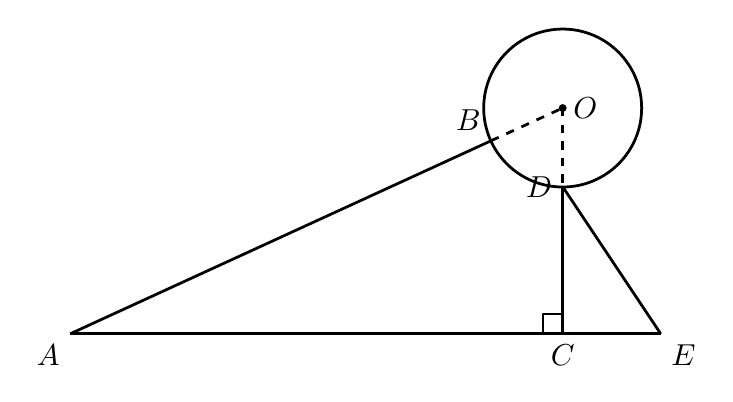
\begin{tikzpicture}[line width=1.0pt, line join=round]
\coordinate (A) at (-3.640,-1.683);
\coordinate (B) at (1.706,0.769);
\coordinate (C) at (2.614,-1.683);
\coordinate (D) at (2.614,0.185);
\coordinate (O) at (2.614,1.184);
\coordinate (U) at (2.363,-1.683);







\coordinate (E) at (3.859,-1.683);


\draw (O) circle (1.003);


\draw (A) -- (C);
\draw (C) -- (E);


\draw (A) -- (B);


\draw[dashed] (B) -- (O);


\draw[dashed] (O) -- (D);


\draw (C) -- (D);


\draw (D) -- (E);


\draw pic[draw, angle radius=0.251cm] {right angle=A--C--D};


\fill (O) circle (0.050cm);


\node[below left, font=\fontsize{10.5}{12.6}\selectfont] at (A) {$A$};
\node[above left, font=\fontsize{10.5}{12.6}\selectfont] at (B) {$B$};
\node[below, font=\fontsize{10.5}{12.6}\selectfont] at (C) {$C$};
\node[left, font=\fontsize{10.5}{12.6}\selectfont] at (D) {$D$};
\node[below right, font=\fontsize{10.5}{12.6}\selectfont] at (E) {$E$};
\node[right, font=\fontsize{10.5}{12.6}\selectfont] at (O) {$O$};
\end{tikzpicture}
\end{document}